\subsection{Command (命令)}

\noindent\textbf{意图}

将一个请求封装为一个对象,从而使你可以用不同的请求对客户进行参数化,对请求排队或记录请求日志,以及支持可撤销的操作。

别名: 动作(action), 事务(transaction)

\noindent\textbf{动机}

假设我们在开发一款文本编辑软件,我们需要通过按钮实现保存功能。那么我们可以将保存的逻辑直接写在按钮的 UI 类中。但是我们也可以使用右键->保存,Ctrl+S 的方式保存文件。显然我们没有必要在这三种方式中都添加保存的逻辑代码。

命令模式即是将某些方法参数化,作为回调函数以达到复用的效果。

\noindent\textbf{适用性}

\begin{itemize}
    \item 抽象出执行的动作以参数化某对象。可用回调函数表示这种参数化机制。
    \item 在不同的时刻指定,排列和执行请求。
    \item 支持取消操作。Command 的 Execute 操作可在实施操作前将状态存储起来,在取消操作时这个状态用来消除该操作的影响。
\end{itemize}

\noindent\textbf{结构}

\begin{figure}[H]
    \scriptsize
    \centering
    \begin{tikzpicture}[scale = 1]
        \begin{class}[text width=2cm]{Client}{0,0}
        \end{class}
        \begin{class}[text width=2cm]{Invoker}{4,0}
        \end{class}
        \begin{interface}[text width=2cm]{Command}{9,0}
            \operation[0]{Execute()}
        \end{interface}
        \begin{class}[text width=2cm]{Receiver}{4,-2}
            \operation{Action()}
        \end{class}
        \begin{class}[text width=3.5cm]{ConcreteCommand}{9,-2.5}
            \implement{Command}
            \operation{Execute(): receiver -> Action()}
            \attribute{state}
        \end{class}
        \aggregation{Invoker}{}{}{Command}
        \draw[umlcd style,fill=white,->] (Client) |- (Receiver);
        \draw[umlcd style,fill=white,->] (ConcreteCommand) -- (Receiver);
    \end{tikzpicture}
\end{figure}

\noindent\textbf{参与者}

\begin{itemize}
    \item \textbf{Command}: 声明执行操作的接口。
    \item \textbf{ConcreteCommand}: 将一个接收者对象绑定与一个动作;调用接收者相应的操作,以实现 Execute。
    \item \textbf{Client}: 创建一个具体命令对象并设定它的接收者。
    \item \textbf{Invoker}: 要求该命令执行这个请求。
    \item \textbf{Receiver}: 知道如何实施与执行一个请求相关的操作。
\end{itemize}

\noindent\textbf{协作}

\begin{itemize}
    \item Client 创建一个 ConcreteCommand 对象并指定它的 Receiver 对象。
    \item 某 Invoker 对象存储该 ConcreteCommand 对象。
    \item 该 Invoker 通过调用 Command 对象的 Execute 操作来提交一个请求。
    \item ConcreteCommand 对象调用它的 Receiver 的一些操作以执行该请求。
\end{itemize}

\begin{figure}[H] 
    \centering 
    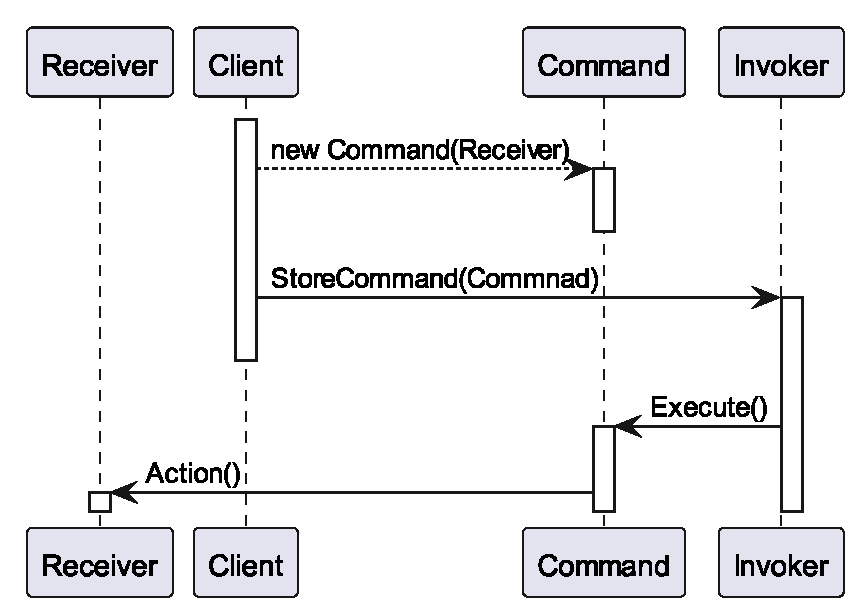
\includegraphics[width=8cm]{figures/Command.eps} 
\end{figure}

\noindent\textbf{优缺点}

\begin{itemize}
    \item Command 模式将调用操作的对象与知道如何实现该操作的对象解耦。
    \item Command 是头等的对象。它们可像其他的对象一样被操纵和扩展。
    \item 可以将多个命令装配成一个组合命令。
    \item 增加新的 Command 很容易,因为着无须改变已有的类。
\end{itemize}

\noindent\textbf{实现}

\begin{itemize}
    \item \textbf{支持撤销(undo)和重做(redo)}: 如果 Command 提供方法逆转它们操作的执行,就可支持撤销和重做功能。为达到这个目的,ConcreteConnamd 类可能需要格外的状态信息。 
\end{itemize}

\noindent\textbf{例子}

\begin{itemize}
    \item Java: \url{https://blog.csdn.net/weixin_40980639/article/details/123218117}
    \item Video: \url{https://www.bilibili.com/video/BV1G5411L7qg}
\end{itemize}

\lstinputlisting[language=Python]{../../scripts/behavioral/Command.py}

\newpage